% !TEX TS-program = pdflatex
% !TEX encoding = UTF-8 Unicode

% This is a simple template for a LaTeX document using the "article" class.
% See "book", "report", "letter" for other types of document.

\documentclass[11pt]{article} % use larger type; default would be 10pt

\usepackage[utf8]{inputenc} % set input encoding (not needed with XeLaTeX)

%%% Examples of Article customizations
% These packages are optional, depending whether you want the features they provide.
% See the LaTeX Companion or other references for full information.

%%% PAGE DIMENSIONS
\usepackage{geometry} % to change the page dimensions
\geometry{a4paper} % or letterpaper (US) or a5paper or....
\geometry{margin=0.5in} 
% \geometry{landscape} % set up the page for landscape
%   read geometry.pdf for detailed page layout information

\usepackage{graphicx} % support the \includegraphics command and options

% \usepackage[parfill]{parskip} % Activate to begin paragraphs with an empty line rather than an indent

%%% PACKAGES
\usepackage{booktabs} % for much better looking tables
\usepackage{array} % for better arrays (eg matrices) in maths
\usepackage{paralist} % very flexible & customisable lists (eg. enumerate/itemize, etc.)
\usepackage{verbatim} % adds environment for commenting out blocks of text & for better verbatim
\usepackage{subfig} % make it possible to include more than one captioned figure/table in a single float
% These packages are all incorporated in the memoir class to one degree or another...

%%% HEADERS & FOOTERS
\usepackage{fancyhdr} % This should be set AFTER setting up the page geometry
\pagestyle{fancy} % options: empty , plain , fancy
\renewcommand{\headrulewidth}{0pt} % customise the layout...
\lhead{}\chead{}\rhead{}
\lfoot{}\cfoot{\thepage}\rfoot{}

%%% SECTION TITLE APPEARANCE
\usepackage{sectsty}
\allsectionsfont{\sffamily\mdseries\upshape} % (See the fntguide.pdf for font help)
% (This matches ConTeXt defaults)

%%% ToC (table of contents) APPEARANCE
\usepackage[nottoc,notlof,notlot]{tocbibind} % Put the bibliography in the ToC
\usepackage[titles,subfigure]{tocloft} % Alter the style of the Table of Contents
\renewcommand{\cftsecfont}{\rmfamily\mdseries\upshape}
\renewcommand{\cftsecpagefont}{\rmfamily\mdseries\upshape} % No bold!

%%% END Article customizations

%%% The "real" document content comes below...

\title{CSU44061 Final Assignment}
\author{17324649 - Efeosa Louis Eguavoen}
%\date{} % Activate to display a given date or no date (if empty),
         % otherwise the current date is printed 

\begin{document}
\maketitle

\section{1}
\subsection{Preprocessing}
The review data we were given was in the form of a JSON in multiple languages.  As the data was in multiple languages and such,  applying machine learning techniques to the data in it's raw for would've proven difficult so some preprocessing was required.  
\\ Initially I considered removing all the removes that were not in English as preprocessing techniques might not work for all the languages in the review data.  I decided against this as just over half of all the reviews in the data were not in English,  and such throwing away that much data would make the final models worse more than likely.  Instead I translated all the non-English reviews to English to get started. 
\begin{verbatim}
def translate_text(text):
    translator = google_translator()
    translation = translator.translate(text)
    origin = text
    translated = translation
    return origin, translated
\end{verbatim}
The above code translates a given review into english and return both the original text and the english version.  I used the Google Translate API to translate into English.
\\ Once the reviews were in English,  I then had to process the data further so it would be in a form that would be usable by the different machine learning techniques I wanted to use.  I started with removing any urls,  emoji's, and numbers from the data.  I also reduced all the words to lower case. 
\begin{verbatim}
def clean_review(review):
    contents = review.lower()
    prepro.set_options(
        prepro.OPT.URL,
        prepro.OPT.EMOJI,
        prepro.OPT.SMILEY,
        prepro.OPT.NUMBER
    )
    clean_contents = prepro.clean(contents)
    contents = clean_contents
    return contents
\end{verbatim}

I then turned the sentences into a list of words or tokens.  I did this so I could then remove all the stop words or words in the english language that don't provide any insight into the meaning of the sentence.  These words occur so frequently also that they don't have any real value hence why I removed them.  Following this,  I lemmatized the tokens.  This process returns a word to it's base.  I chose this over stemming as it's more intelligent as stemming just removes the start or end of a word while lemmatization takes into account the meaning of the word and returns the lemma of it or the dictionary version of the word.
\begin{verbatim}
def tokenize(review):
    tokens = word_tokenize(review)
    stop_words = set(stopwords.words("english"))
    useful_tokens = []
    lemma = WordNetLemmatizer()
    for token in tokens:
        if (not token in stop_words) and (token.isalpha()):
            lemmatnised_token = lemma.lemmatize(token)
            useful_tokens.append(lemmatnised_token)
    return useful_tokens
\end{verbatim}
\subsection{Methods and Hyperparameter Selection}
To see if the review data could 1) Predict the review Polarity and 2) determine if it was in early access or not,  I evaluated 2 very different machine learning models,  A Support Vector Classifier and Convolutional Neural Network.  
\subsubsection{Support Vector Classifier}
A SVC is a supervised machine learning method that tries to find the line that separates the data into it's respective classes,  or the decision boundary.  The main difference between this and Logistic regression is in the loss function, with a SVC using a hinge-loss function.  I went with this method as I wasn't sure if my data was going to be linearly separable as it wasn't numerical data.  SVC's can use non-linear kernels that would adapt better to non-linear data. 
\\ To make the data usable in a SVC  I did a little more preprocessing on the data.  I turned the reviews into a series of vectors using the Term-Frequency and Inverse Document Frequency method or TF-IDF method.  I chose this as using word counts and such was too basic and can be weighted down by words with high frequency and hence lose interesting words in the data.  TF-IDF is better as it prioritises the words in each document so words that occur frequently between documents end up being weighted less as a result of their frequency while words that don't repeat as often are weighted more. 
\begin{verbatim}
def tf_idf(dataset):
    data = dataset["tokens"].values
    tfidf_converter = TfidfVectorizer(min_df=5, max_df=0.7)
    wordDoc = [" ".join(x) for x in data]
    X = tfidf_converter.fit_transform(wordDoc)
    y = dataset["Voted Up"].values
    # df = pd.DataFrame(X[0].T.todense(), index=tfidf_converter.get_feature_names(), columns=["TF-IDF"])
    # df = df.sort_values('TF-IDF', ascending=False)
    # print(df.head())
    return X, y
\end{verbatim}

There are a 3 main hyperparameters to chose for the SVC,  C or how serve a penalty the regulizer gives,  the kernel that's used and Gamma or how muc h influence each point in the data exerts on other points in the dataset. 
\\Given that there's a large number of hyperparameters,  I started with a Gridsearch of the combinations.  I defined a few values of C,  the different kernels I could use and then different Gamma values and evaluated them in terms of Accuracy on the dataset.  This gave me a kind of starting point to tune the data further as I could narrow down the kernel to use.  
\begin{verbatim}
def hyper_pick(X, y):
    """
    Select the best parameters and hyperparameters for the training data using GridSearchCV
    :param X: Tf-IDF scores of tweet data
    :param y:Sentiment values of the tweets
    :return: Outputs a graph of data
    """
    X_train, X_test, y_train, y_test = train_test_split(X, y, test_size=0.2, random_state=101)
    param_grid = [{'C': [0.01, 0.1, 1, 10, 100], 'gamma': [10, 1, 0.1, 0.01, 0.001],
                   'kernel': ['rbf', 'poly', 'sigmoid']}, {'kernel': ['linear'], 'C': [0.01, 0.1, 1, 10, 100],
                                                           'gamma': [10, 1, 0.1, 0.01, 0.001]}]
    grid = GridSearchCV(SVC(), param_grid, refit=True, verbose=2, n_jobs=-1, scoring='accuracy')
    grid.fit(X_train, y_train)
    print(grid.best_params_)
\end{verbatim}
From here I tuned the K and C parameters using 5-fold cross validation.  This outputed a graph so I could then chose an optimal value of K and C. 
\begin{verbatim}
def cross_val(k, model, X, y):
    """
    Inputs: kfold number, machine learning model, data to evaluate X,y

    Outputs: The accuracy, recall and precision and their respective standard deviations for the model
    """
    accuracy_list = []
    recall_list = []
    precision_list = []
    labels = [0, 1]
    kf = KFold(n_splits=k)
    for train, test in kf.split(X):
        model.fit(X[train], y[train])
        predict = model.predict(X[test])

        accuracy = accuracy_score(y[test], predict)
        recall = recall_score(y[test], predict, labels=labels, average='macro')
        precision = precision_score(y[test], predict, labels=labels, average='macro')
        accuracy_list.append(accuracy)
        recall_list.append(recall)
        precision_list.append(precision)

    accuracy_end = np.mean(accuracy_list)
    std = np.std(accuracy_list)
    recall = (np.mean(recall_list), np.std(recall_list))
    precision = (np.mean(precision_list), np.std(precision_list))

    print('Accuracy: ', accuracy_end)
    print('Standard Deviation', std)
    print('Recall', recall)
    print('Precision', precision)

    return accuracy_end, std, recall, precision


def plot_accuracy(X, y):
    """
    Purpose:
        Plots the accuracy and standard deviation for different gamma, C
        Using to fine tune these parameters
    """
    gamma = [0.1, 1, 10, 100]
    C = [0.1, 1, 10, 100]
    plotx = [0, 1, 0, 1]  # lists for plotting
    ploty = [0, 0, 1, 1]  # lists for plotting
    gs = GridSpec(2, 2, wspace=0.3, hspace=0.3)
    fig = plt.figure(figsize=(20,10))
    l = 0
    for i in gamma:

        gx = plotx[l]
        gy = ploty[l]
        ax = fig.add_subplot(gs[gx, gy])
        accuracy_list = []
        std_list = []
        for c in C:
            model = SVC(kernel='sigmoid', gamma=i, C=c)
            accuracy, std, _, _ = cross_val(5, model, X, y)
            accuracy_list.append(accuracy)
            std_list.append(std)
        plt.errorbar(C, accuracy_list, yerr=std_list)
        ax.set_title('Gamma = ' + str(i))
        ax.set_ylabel('Accuracy')
        ax.set_xlabel('C')
        plt.xscale('log')
        l = l + 1
    plt.tight_layout()
    plt.show()
\end{verbatim}
\begin{figure}[h]
\centering
\subfloat[Voted Up]{{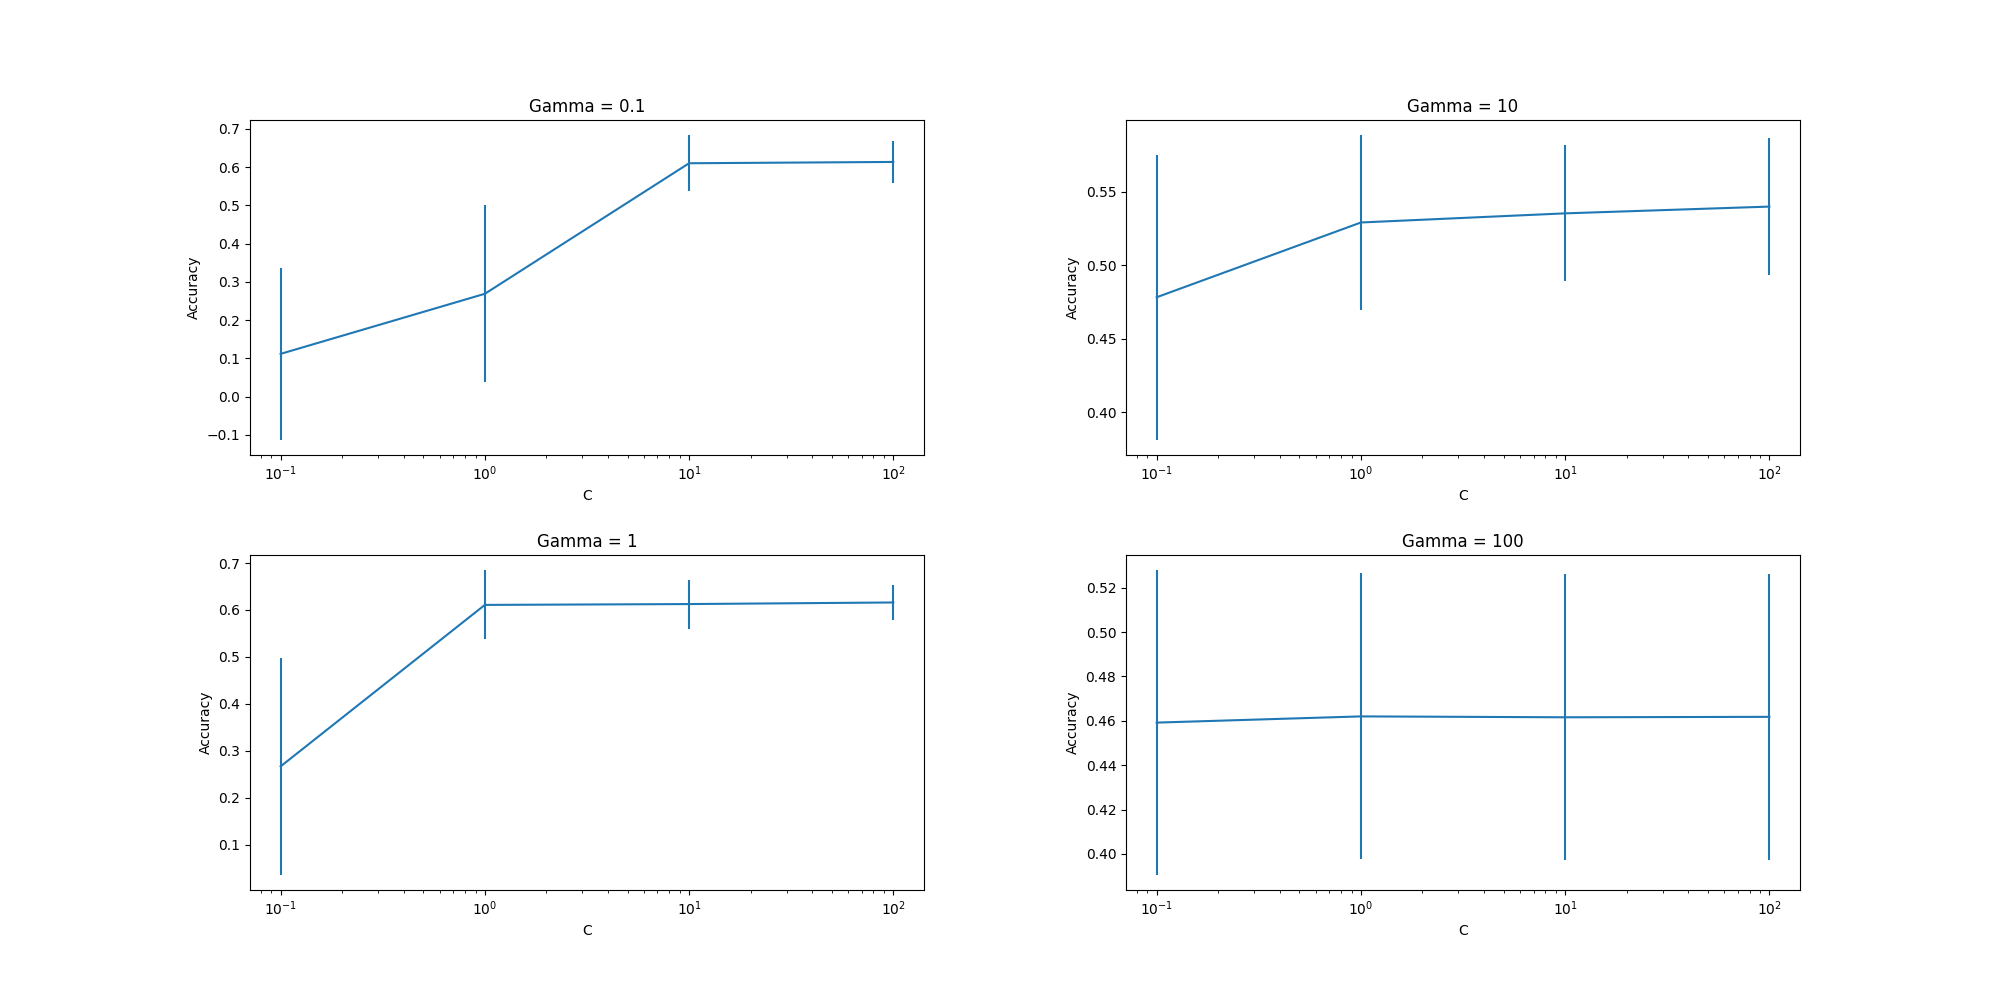
\includegraphics[width=18cm]{myplot.png}}}
\qquad
\subfloat[Early Access]{{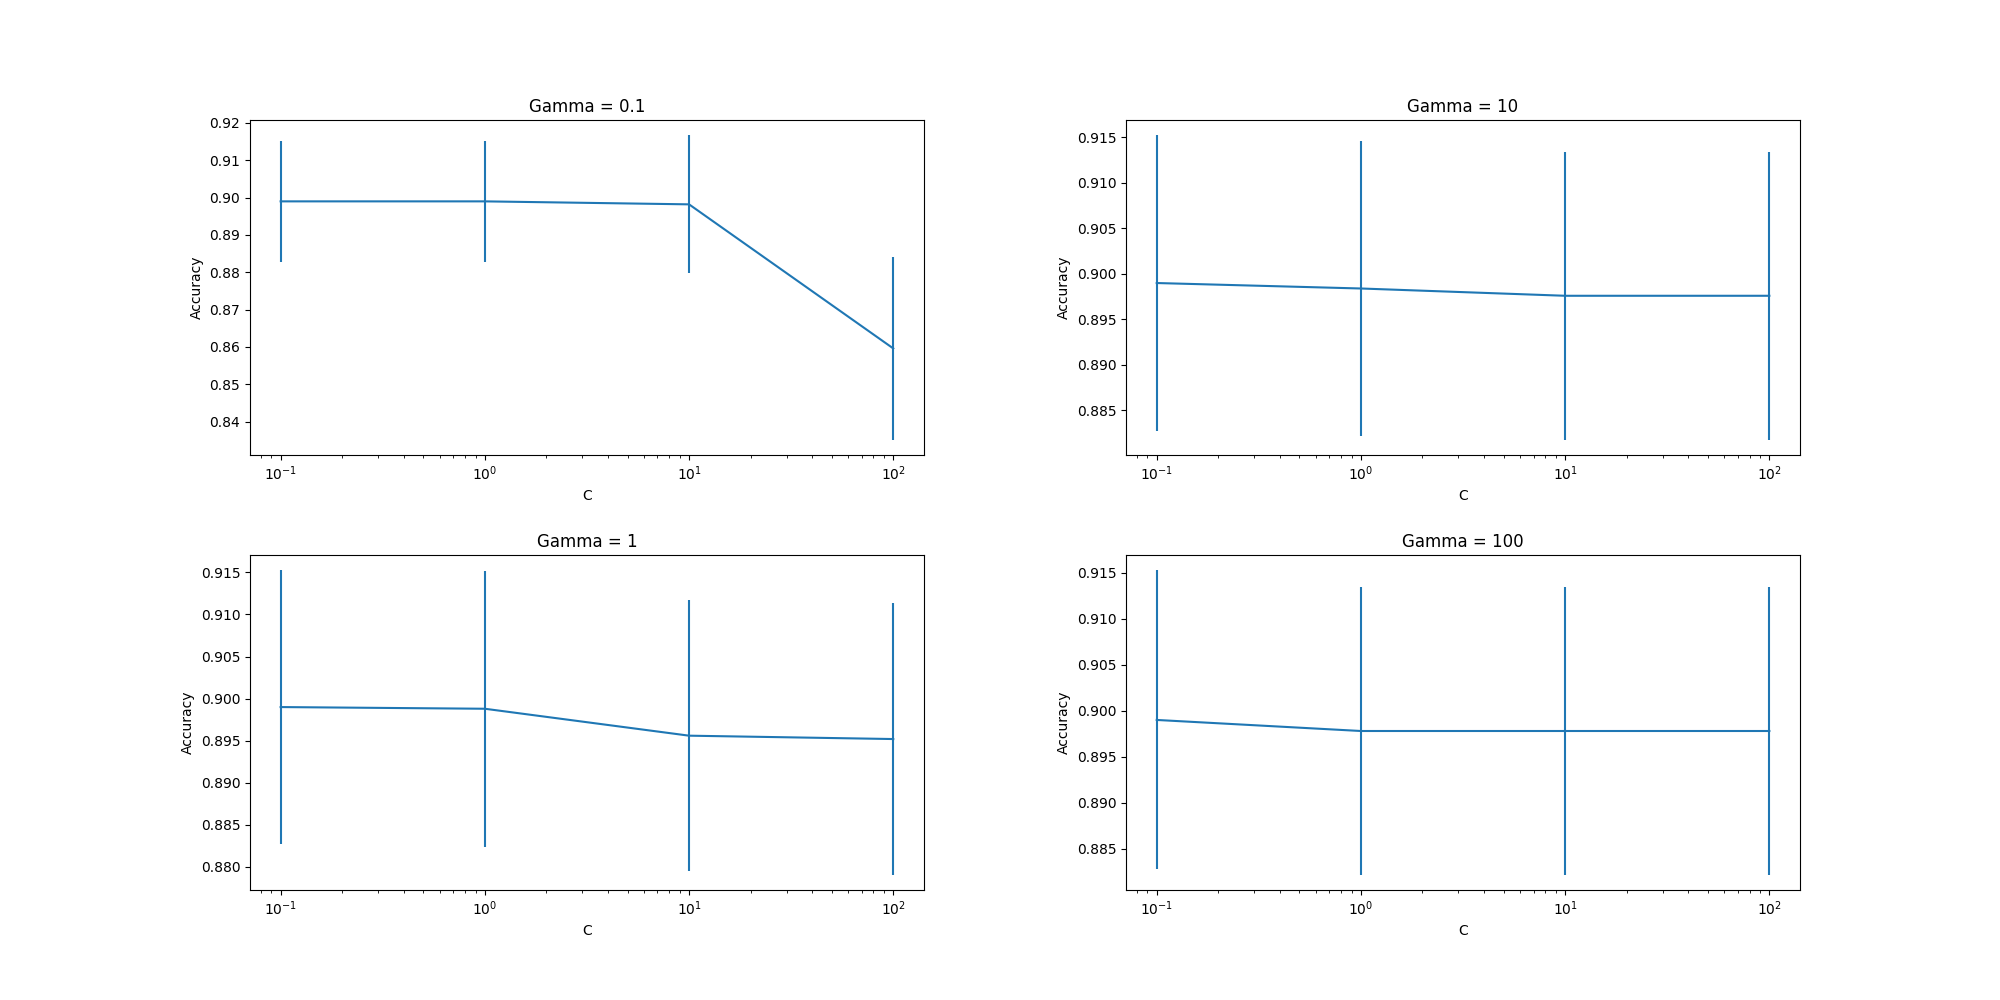
\includegraphics[width=18cm]{eacv.png}}}
\end{figure}

From the above graphs we can see that when C =1 and Gamma = 1 also we can maximise the accuracy so those are the hyper parameters I chose for 'Voted Up'.  From using GridSearchCV,  we found that using a Sigmoid kernel was the best fit for the data. 
\\ For 'Early Access' the graphs indicate that when Gamma = 0.1 and C = 0.1 with a Gaussian kernel seems to be the best combination of hyper-parameters. 
\subsubsection{Convolutional Neural Network}
For the deep learning algorithms,  I had to go with a different approach for using the text data.  Instead of doing One-Hot Encoding with the TF-IDF vectorizer,  I instead went with a word embedding approach as deep learning needs to know the association between words to make accurate predictions.\\To do this, I made use of the preprocessed texts but used a tokenizer that turned our text corpus into a series of vectors. 
\begin{verbatim}
tokenizer = Tokenizer(num_words=len(TRAINING_VOCAB), lower=True, char_level=False)
    tokenizer.fit_on_texts(train_data["Text_Final"].tolist())
    training_sequences = tokenizer.texts_to_sequences(train_data["Text_Final"].tolist())
\end{verbatim} 
Following this I used Google’s word2vec for word associations since our vocabulary size wasn’t large enough for us to train my own embeddings. For each of our models, I added an embedding layer that acted as our input layer for the vectors.
\begin{verbatim}
train_word_index = tokenizer.word_index
    print('Found %s unique tokens.' % len(train_word_index))
    train_embedding_weights = np.zeros((len(train_word_index) + 1, EMBEDDING_DIM))
    for word, index in train_word_index.items():
        train_embedding_weights[index, :] = word2vec[word] if word in word2vec else np.random.rand(EMBEDDING_DIM)
\end{verbatim}
In terms of hyperparameters,  there's numerous ones to train such as the embedding dimensions size,  the number of convolutional layers we should use,  the batch size we should use for training and numerous others. Tuning all these hyperparameters using cross validation was too time intensive, so instead I focused on cleaning the data better as it provided a more immediate improvement and took much less time to do.  I did attempt to find the optimum amount of Epochs to run the CNN for. 
\begin{figure}[h]
\centering
\subfloat[Voted Up]{{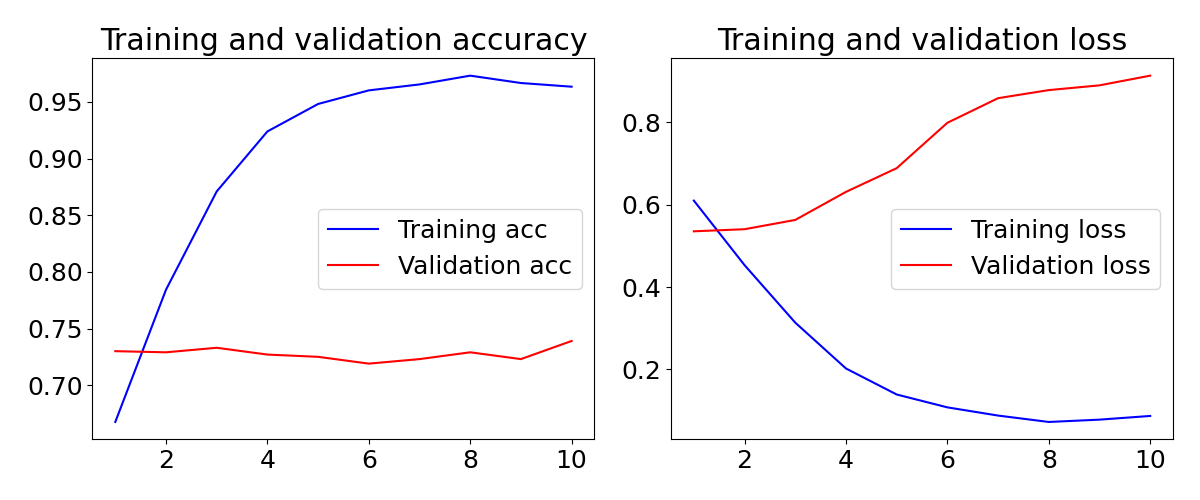
\includegraphics[width=13cm]{vupcnn.png}}}
\qquad
\subfloat[Early Access]{{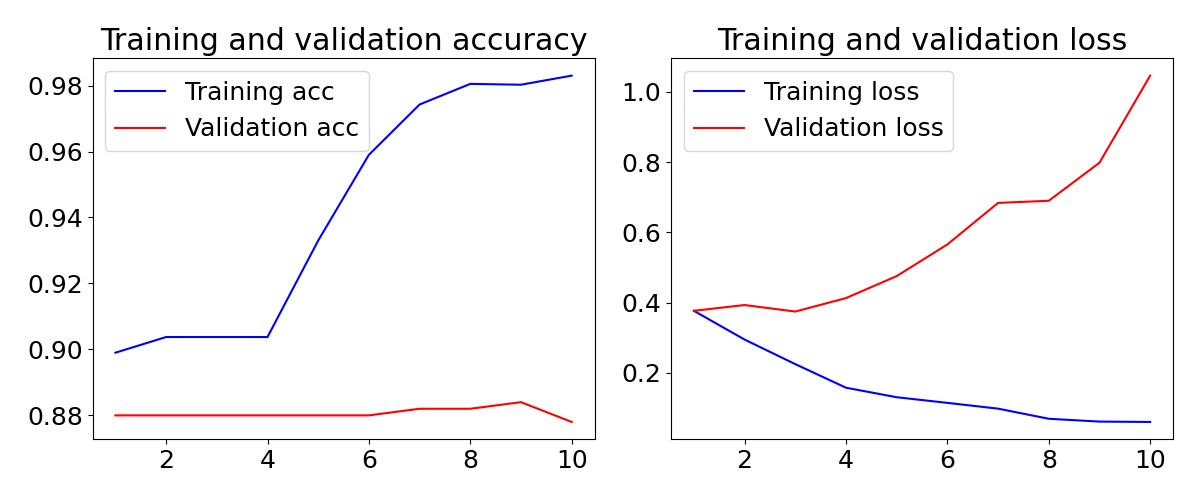
\includegraphics[width=13cm]{eacnn.png}}}
\end{figure}
From the above figures,  training the data for about 3 epochs seems to be the best tradeoff between accuracy and loss for 'Voted Up'
\\ Similarly,  for 'Early Access' it seems about 3 epochs is the sweet spot between accuracy and loss.
\subsection{Results}
\end{document}
